\documentclass[a4paper, 10pt]{article}

\usepackage[utf8]{inputenc}
\usepackage[T1]{fontenc}
\usepackage[french]{babel}
\usepackage{listings}
\usepackage{amsmath}
\usepackage{graphicx}
\usepackage[top=2.5cm,bottom=2.5cm,right=2.5cm,left=2.5cm]{geometry}


\title{\Huge{TP Carte}}
\author{Jules HABLOT \and Rémi GATTAZ \and Anna BRUEL}
\date{\today}

\begin{document}
\maketitle

\begin{figure}[hc]
	\centering
	
\includegraphics[scale=2.5]{logo_pg.png}
\end{figure}

\begin{figure}[hbc]
	\centering
	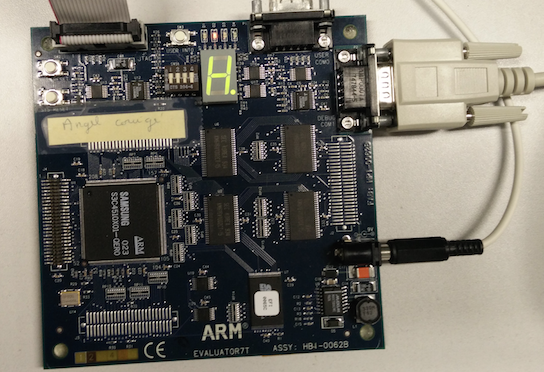
\includegraphics[scale=1.40]{carte2}
\end{figure}

\clearpage

\section{Fonctionnalités atteintes}

Nous allons vous présenter les diverses fonctionnalités que nous avons implémenté et comment les utiliser. Nous avons choisi de commencer le TP Carte par l'utilisation de la liaison série. Nous nous sommes donc très vite intéressés à la gestion d'une interruption. Ensuite, nous avons essayé de faire quelque chose avec l'afficheur 7 segments dans le temps où le programme attend un interruption. Enfin nous voulions faire un affichage du message reçu par la liaison série sur le 7 segment en le faisant défiler à l'aide du bouton poussoir.

\subsection{Interruption}

Lors d'une interruption, le code assembleur à l'étiquette \textit{\_irq\_handler} est exécuté. Après la sauvegarde des registres, la fonction \textit{traiter\_interruption} dans notre programme est appelée.

Dans cette fonction, nous gérons deux interruptions différentes : l'arrivée d'un message sur la ligne série et l'utilisation du bouton pressoir. Pour cela faisons un test pour connaitre le type d'interruption qui a été déclenchée. C'est une fois que la source de l'interruption est déterminée que l'appel au traitant d'interruption correspondant est effectué.

\subsubsection{Transfert de string}

Il s'agit de l'interruption due à un transfert de bits, la carte reçoit des bits par la ligne série et génère une interruption pour chaque caractère reçu. Le traitant d'interruption va lire tout le message envoyé et le stocker dans un tableau. C'est plus tard, dans le programme principal que nous allons l'utiliser. Dans le cas où le tableau est plein, les interruptions futures sont bloquées. Ainsi pour lire tout le message, il faut plusieurs fois passer dans le traitant d'interruption, une fois par caractère. De plus pour marquer la fin de l'envoi et la fin du message, nous définissons une marque de fin, le point \textit{"."} . Si un nouveau message arrive sur la liaison série pendant que le premier est en lecture sur le 7 segment, le deuxième prendra la place mémoire du premier et l'effacera.

\subsubsection{Bouton poussoir}

Le bouton pressoir permet de changer la lettre du message à afficher sur le 7 segments. Lors de l'appui sur ce bouton, une interruption est levée et notre programme change la lettre à afficher. Cette deuxième interruption n'est pas prioritaire, si la carte reçoit un message et que l'on appuie sur le bouton en même temps c'est le message qui sera lu avant la gestion du bouton. Ceci est dû au fait que dans la fonction testant quel traitant d'interruption doit être appelée, le test pour l'interruption ligne série est effectué avant.

\subsection{Affichage}

Nous voulions faire des affichages pour voir concrètement où en est notre programme. Nous avons donc définie une boucle d'attente, il s'agit d'une simple boucle qui affiche le signe de l'infini sur les 7 segments, et qui tourne en boucle. Cette boucle est notre boucle principale, lors du lancement du programme sur la carte, cette boucle commence et continue jusqu'à une interruption ou l'arrêt de la carte. L'interruption peut être l'arrivée d'un message à lire, dans ce cas le message est lu puis la première lettre de ce message est affichée. L'autre interruption consiste à la pression du bouton, c'est pour avancer dans le message et afficher la lettre suivante. Aussi, le nombre de lettres qu'il reste à afficher avant la fin du message est écrit en binaire par le biais des 4 LEDs de la carte.

\subsubsection{LEDs}

Nous avons implémenté une simple fonction qui, recevant un entier en base 10, affiche en base 2 ce nombre à l'aide des LEDs. Puisque nous n'avons que 4 LEDs, ce nombre est affiché modulo 16.

\subsubsection{7 segments}

Nous utilisons l'afficheur 7 segments pour afficher notre boucle infinie en continue dans notre programme principale, mais nous affichons aussi les lettres du message, nous avons implémenté toutes les lettres de l'alphabet. Néanmoins le message ne doit contenir que des minuscules et étant donnée que l'afficheur est un 7 segments, certaines lettres de l'alphabet sont méconnaissables.

\subsection{Pour aller plus loin}

Pour notre boucle de l'infini nous utilisons un compteur qui s'incrémente par addition successive. Il nous manquerait d'utiliser un timer pour faire changer d'état notre affichage. Nous avons entendu que le timer ne faisait qu'incrémenter un registre et que pour simplifier nous pouvions faire cet incrément dans une boucle en dur, mais nous voudrions utiliser le timer pour gérer une FIQ et ainsi avoir fait tout le possible avec notre carte.

\section{Organisation logicielle}

Afin de permettre une réutilisabilité de certaines parties du programme, nous avons décidé de créer un fichier pour chaque composant que nous utilisons sur la carte. Pour cette même raison, nous avons pour chaque composant produit des fonctions qui n'ont pas d'autres effets de bords que celui attendu comme résultat de la fonction. Ainsi, nous avons créé les fichiers suivants :
\newline
\begin{itemize}

	\item {\bfseries affichage\_7Segs.c} : Contient les fonctions gérant le 7 segments. Il contient deux fonctions d'affichage et une procédure pour éteindre tous les segments. Les fonctions d'affichage permettent d'imprimer toutes les lettres de l'alphabet et de faire une boucle affichant le symbole infini.
	\newline
	\item {\bfseries affichage\_LEDs.c} : Contient les fonctions gérant les LEDs. Cela inclut une procédure pour éteindre toutes les diodes et une fonction affichant un nombre en base 2 modulo 16 avec l'aide des 4 LEDs.
	\newline
	\item {\bfseries ligneSerie.c} : Contient les fonctions permettant l'utilisation de la liaison série. Il contient les fonctions \textit{readByte} et \textit{writeByte} permettant de lire ou écrire un caractère sur la liaison série.
	\newline
	\item {\bfseries main.c} : Il s'agit du fichier contenant le programme principal
\end{itemize}

\vspace{.8em}

Seuls les traitant d'interruptions et quelques fonctions utilitaires ne sont pas séparés du programme principal. Nous avions à la base prévu d'avoir un fichier interruption.c contenant ces fonctions mais nous avions des problèmes à partager des variables globales entre fichiers. Nous avons donc finalement fait ce choix.

\end{document}

